\chapter{Конструкторская часть}

\section{Последовательность преобразований}

На рисунках~\ref{idef00}~и~\ref{idef01} представлены IDEF0-диаграммы разрабатываемого загружаемого модуля ядра.
\begin{figure}[H]
	\centering
	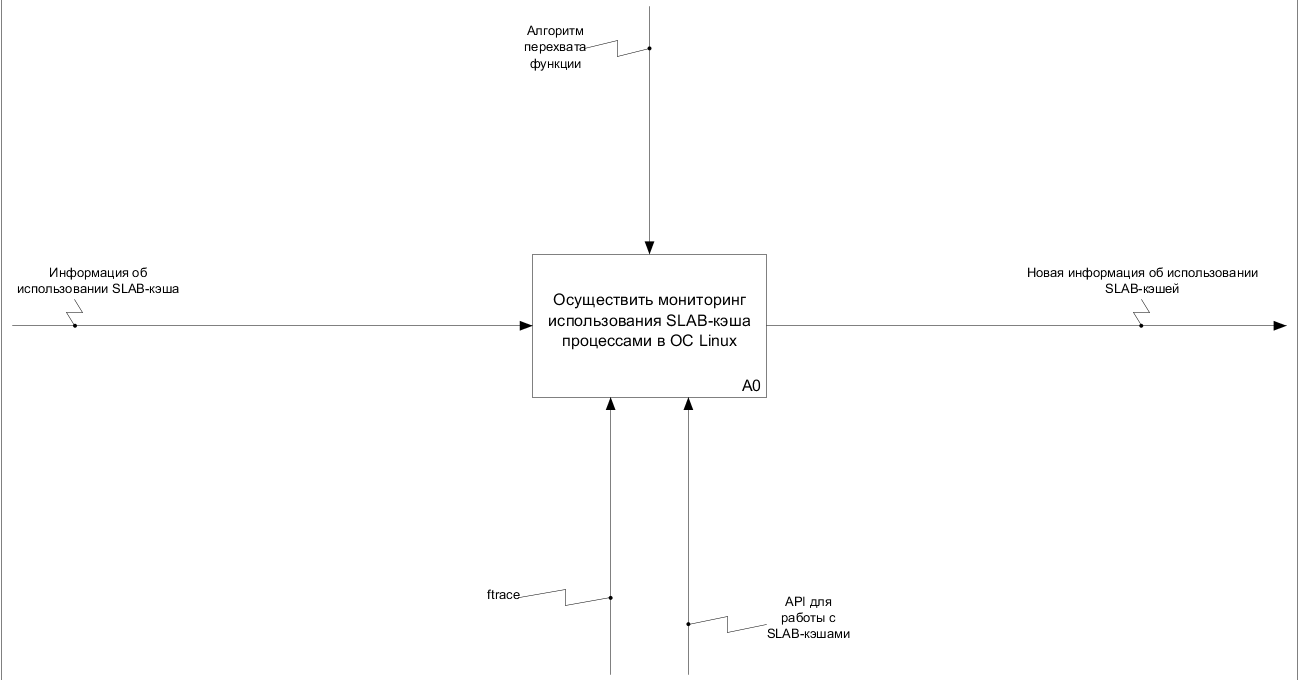
\includegraphics[width=\linewidth]{idef00}
	\caption{IDEF0-диаграмма нулевого уровня}
	\label{idef00}
\end{figure}
\begin{figure}[H]
	\centering
	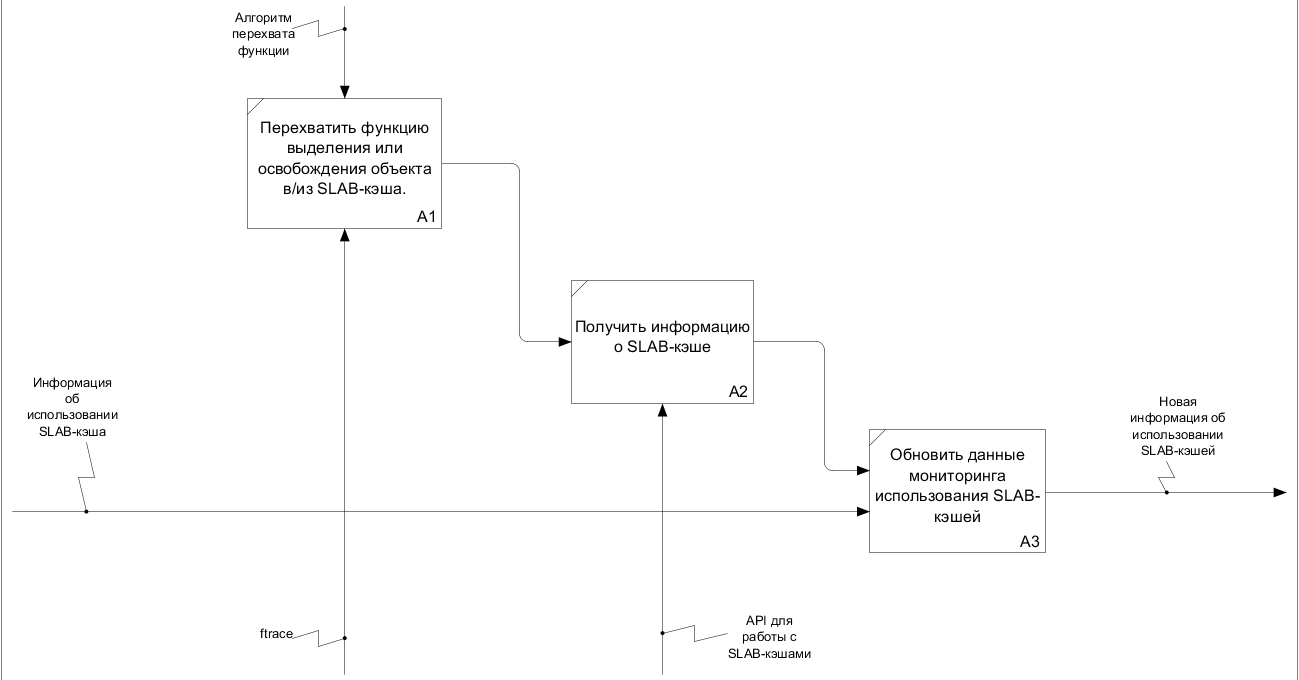
\includegraphics[width=\linewidth]{idef01}
	\caption{IDEF0-диаграмма первого уровня}
	\label{idef01}
\end{figure}

\section{Алгоритм загрузки и выгрузки загружаемого модуля ядра}

На рисунке~\ref{init_exit_alg} представлены схемы алгоритмов загрузки и выгрузки загружаемого модуля ядра.
\begin{figure}[H]
	\centering
	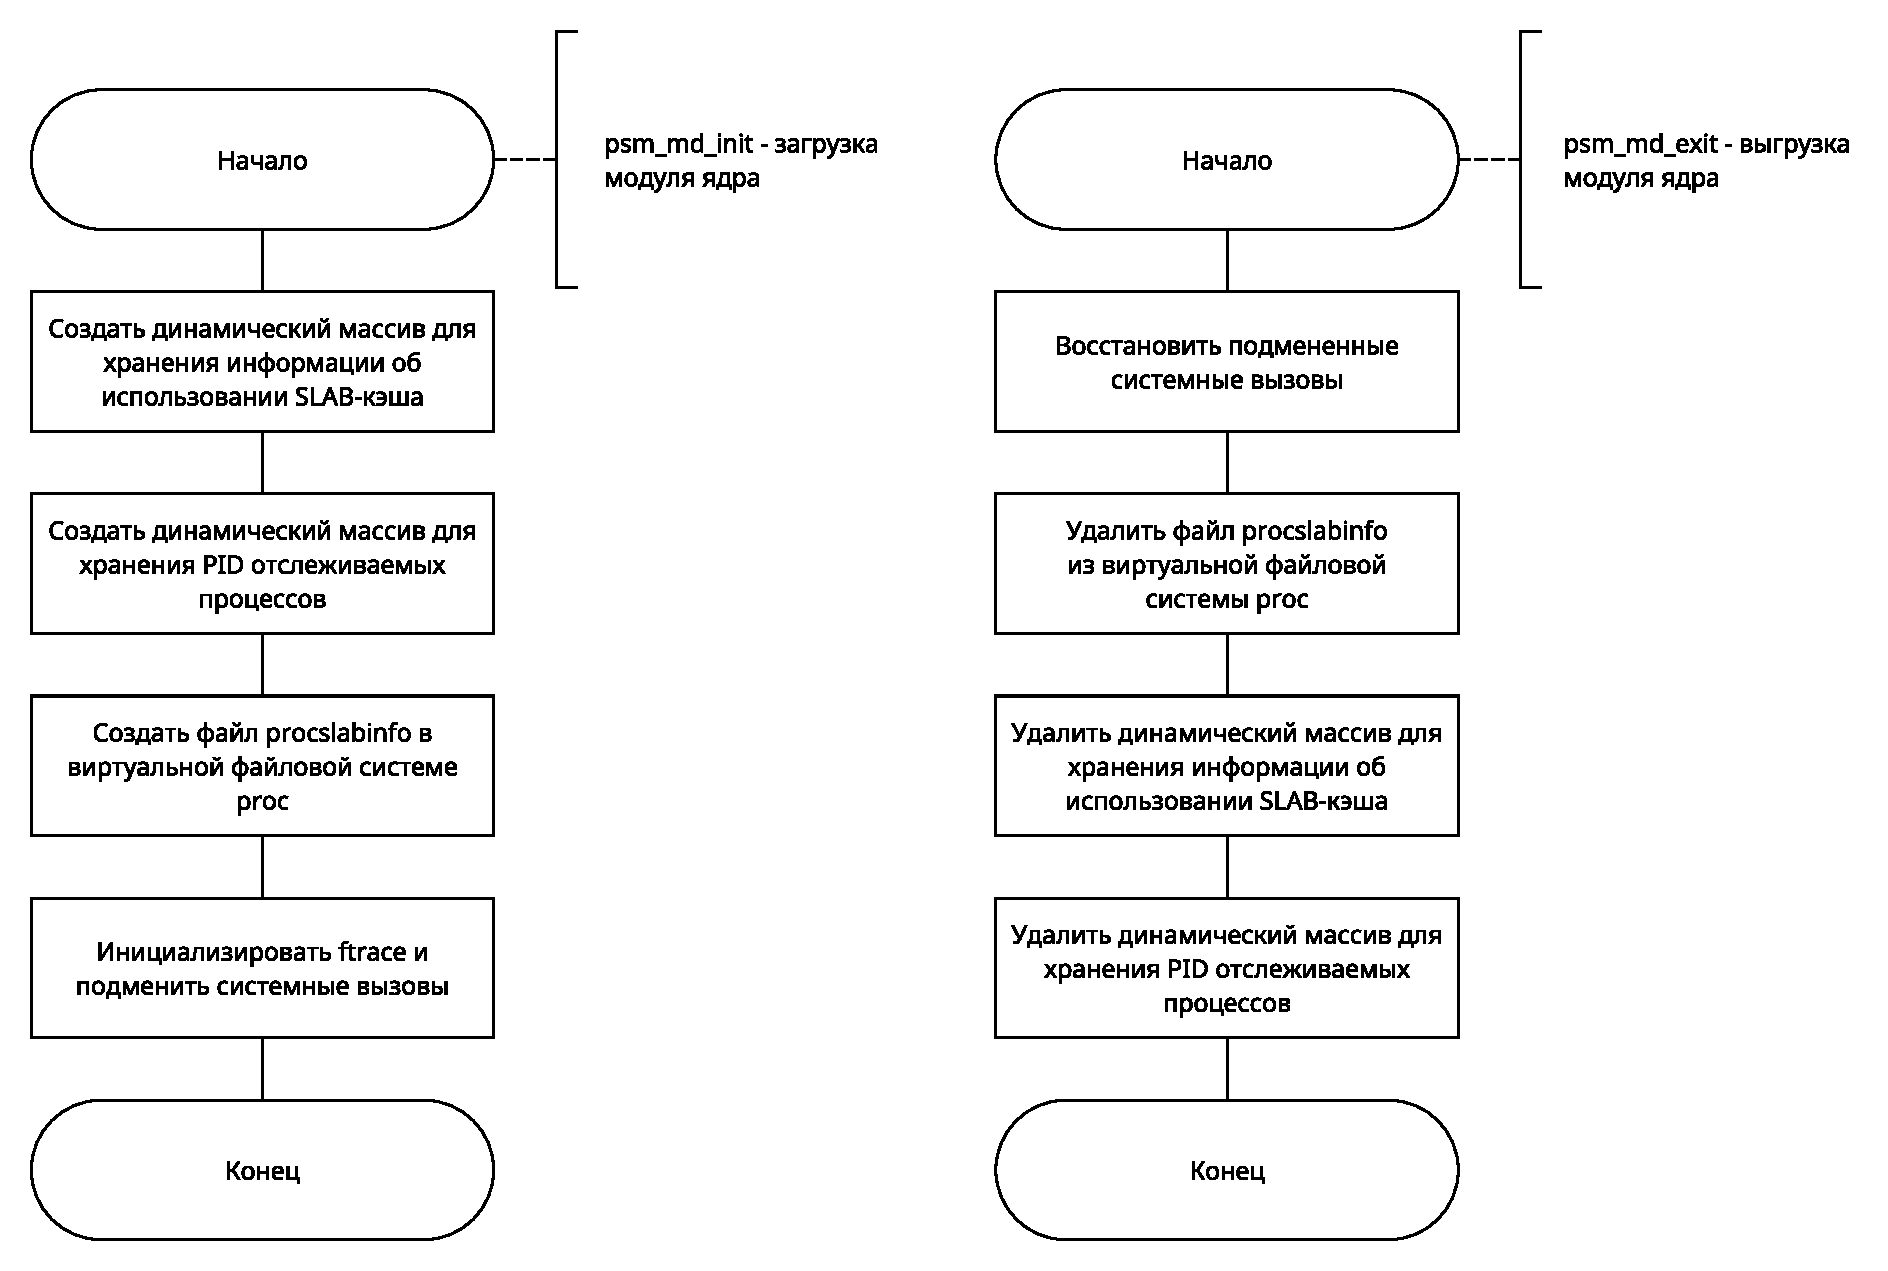
\includegraphics[width=\linewidth]{init_exit_alg}
	\caption{Схемы алгоритмов загрузки и выгрузки загружаемого модуля ядра}
	\label{init_exit_alg}
\end{figure}

\section{Алгоритм перехвата функции ядра}

На рисунке~\ref{ftrace_alg} представлена схема алгоритма перехвата функции ядра.
\begin{figure}[H]
	\centering
	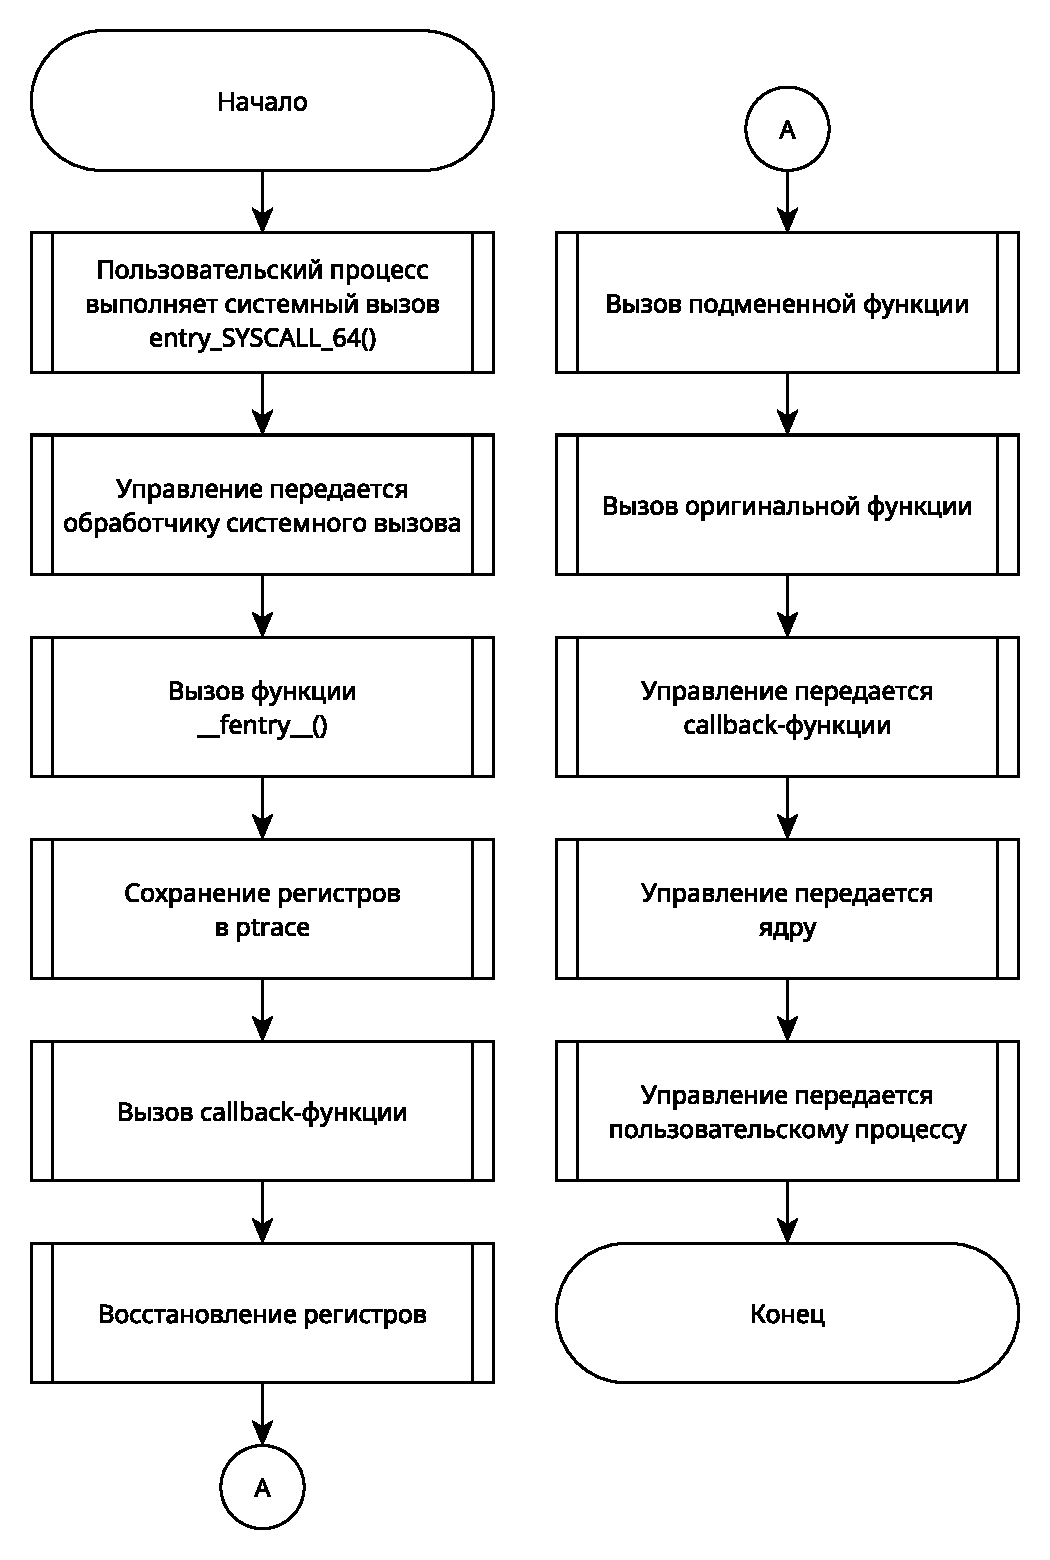
\includegraphics[width=0.5\linewidth]{ftrace_alg}
	\caption{Схема алгоритма перехвата функции ядра}
	\label{ftrace_alg}
\end{figure}

\section{Алгоритмы чтения и записи для файла в виртуальной файловой системе proc}

На рисунках~\ref{proc_read_alg}~и~\ref{proc_write_alg} представлены схемы алгоритмов чтения и записи для файла в виртуальной файловой системе proc соответственно.
\begin{figure}[H]
	\centering
	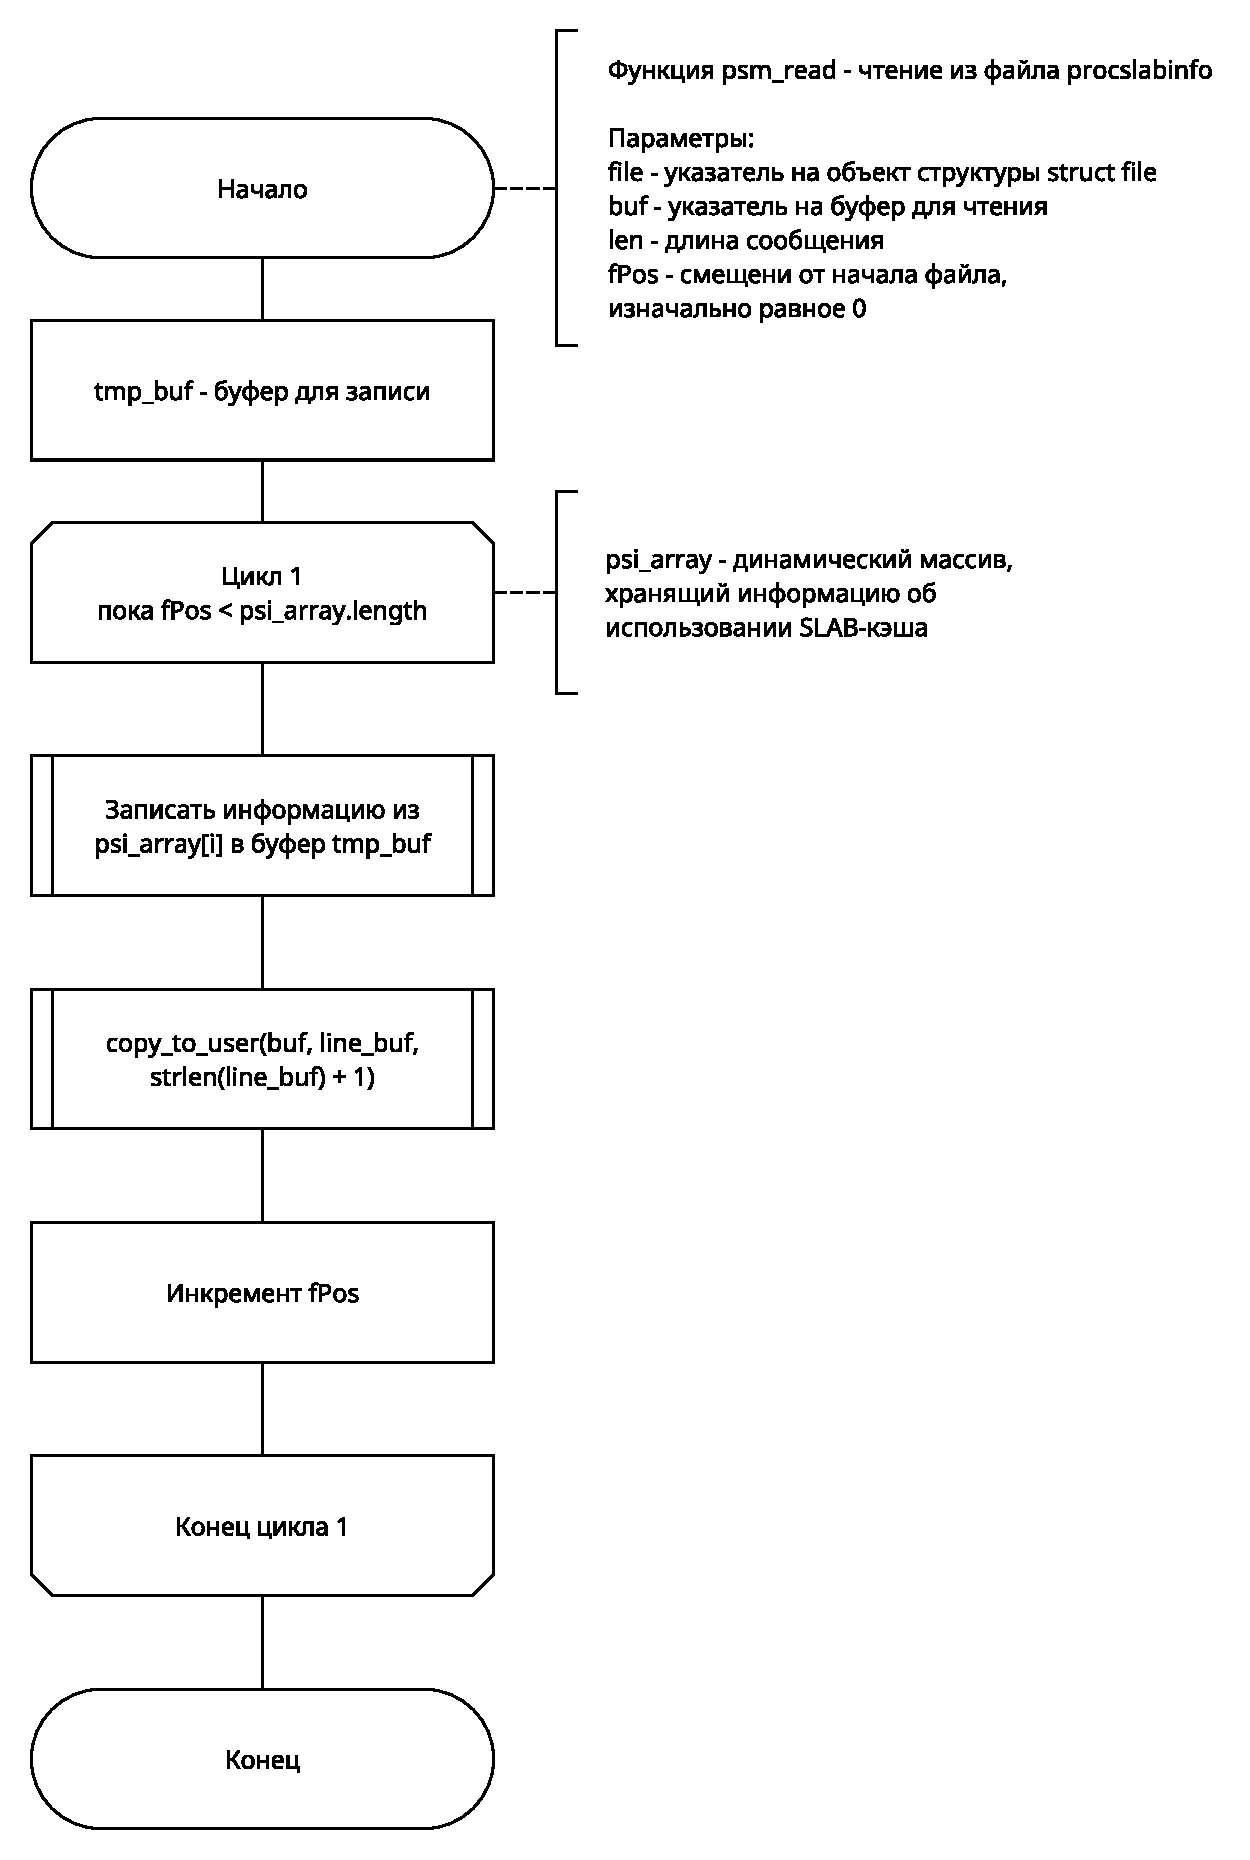
\includegraphics[width=0.5\linewidth]{proc_read_alg}
	\caption{Схема алгоритма чтения из файла в виртуальной файловой системе proc}
	\label{proc_read_alg}
\end{figure}
\begin{figure}[H]
	\centering
	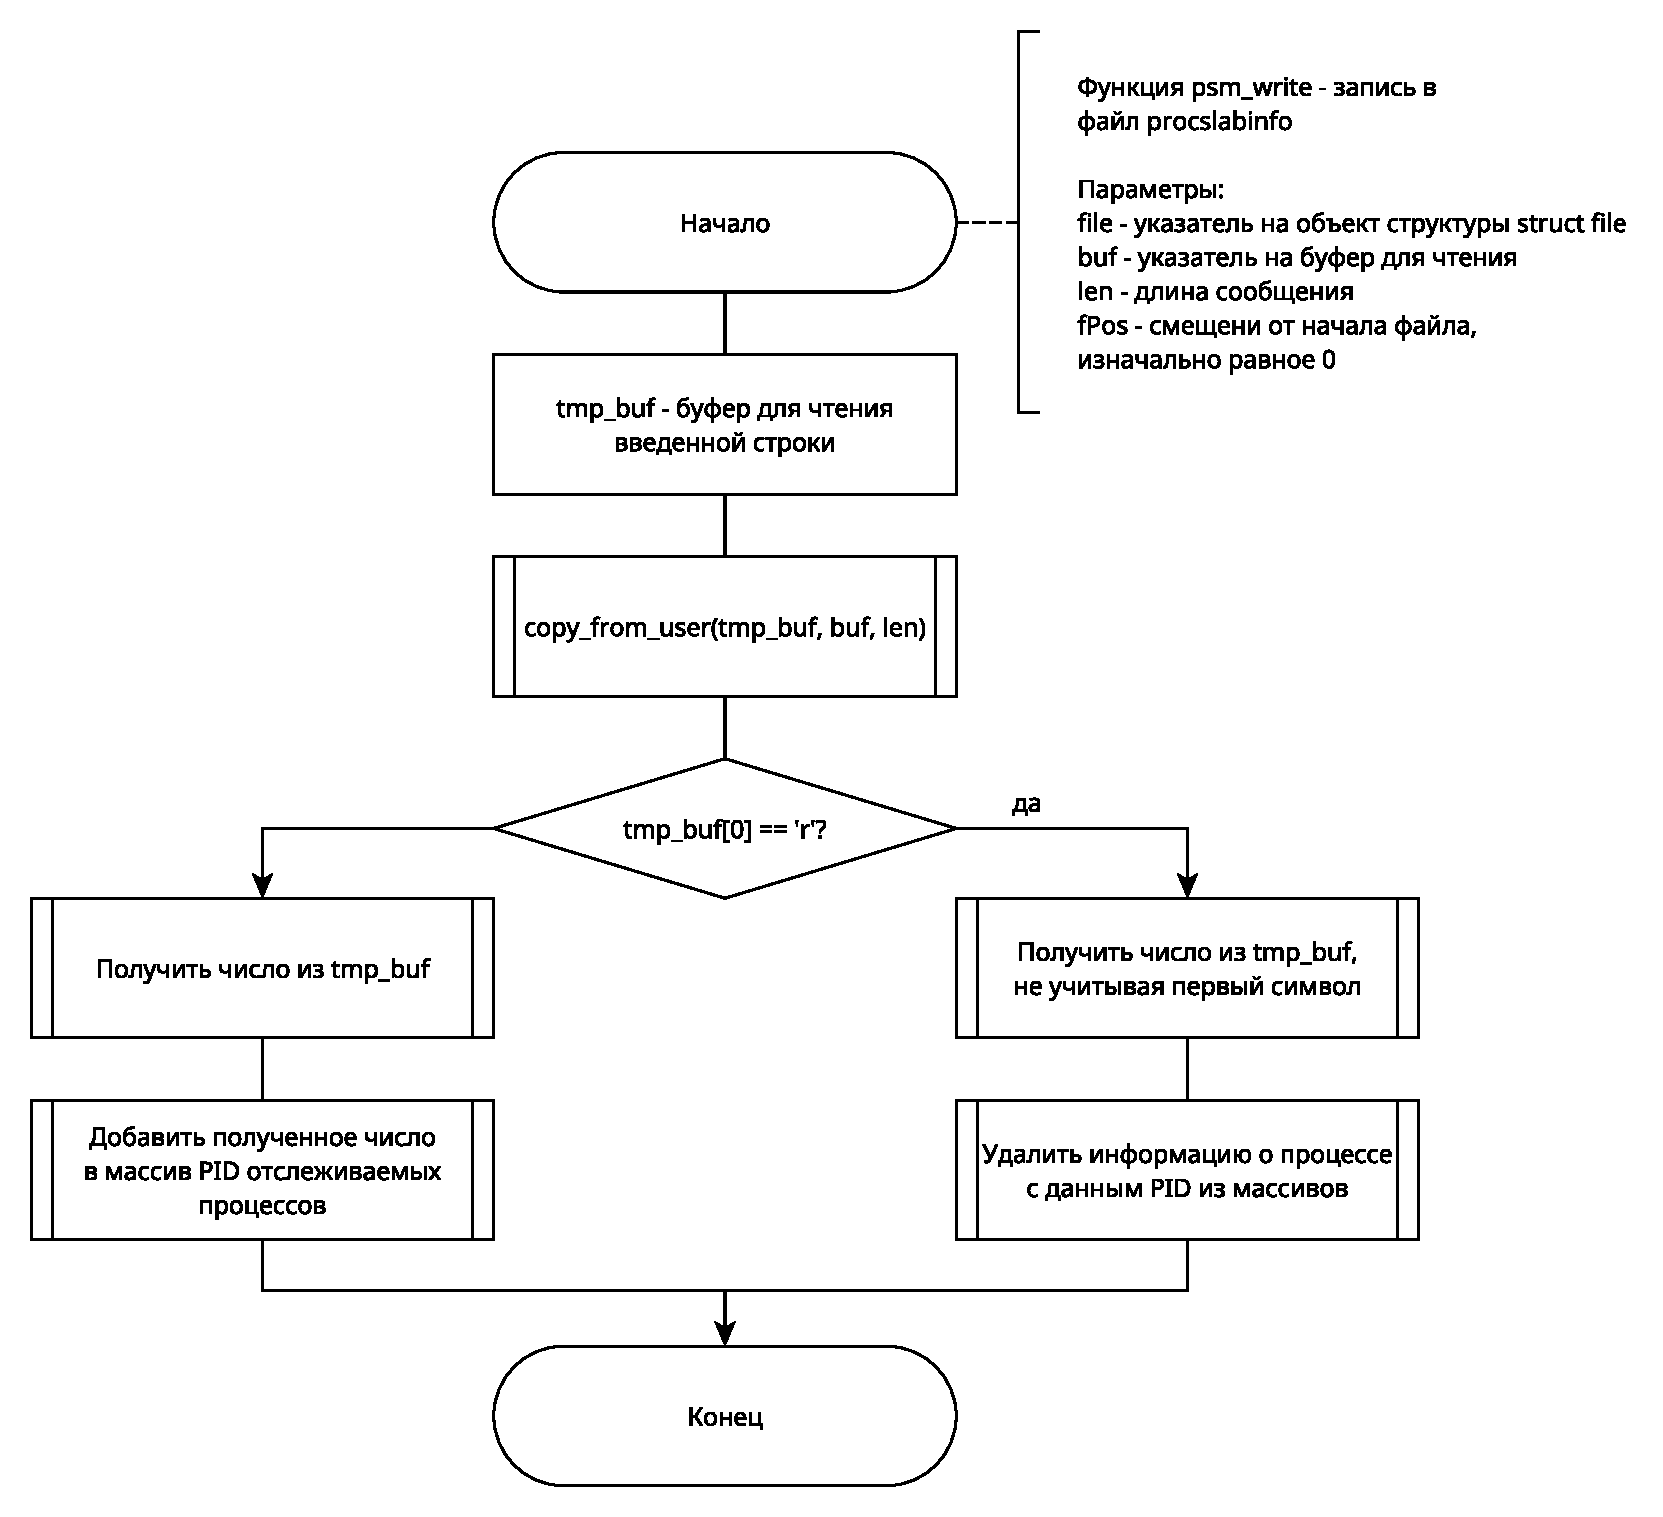
\includegraphics[width=0.6\linewidth]{proc_write_alg}
	\caption{Схема алгоритма записи в файл в виртуальной файловой системе proc}
	\label{proc_write_alg}
\end{figure}

\section{Алгоритмы подменяемых функций}

На рисунках~\ref{fh_in_kmem_cache_alloc_node_alg}~--~\ref{fh_kmem_cache_destroy_alg} представлены алгоритмы подменяемых функций. Схемы алгоритмов процедур commit\_kmem\_cache\_alloc, commit\_kmem\_cache\_free, commit\_kmem\_cache\_destroy представлены на рисунках~\ref{commit_kmem_cache_alloc_alg}~--~\ref{commit_kmem_cache_destroy_alg}.
\begin{figure}[H]
	\centering
	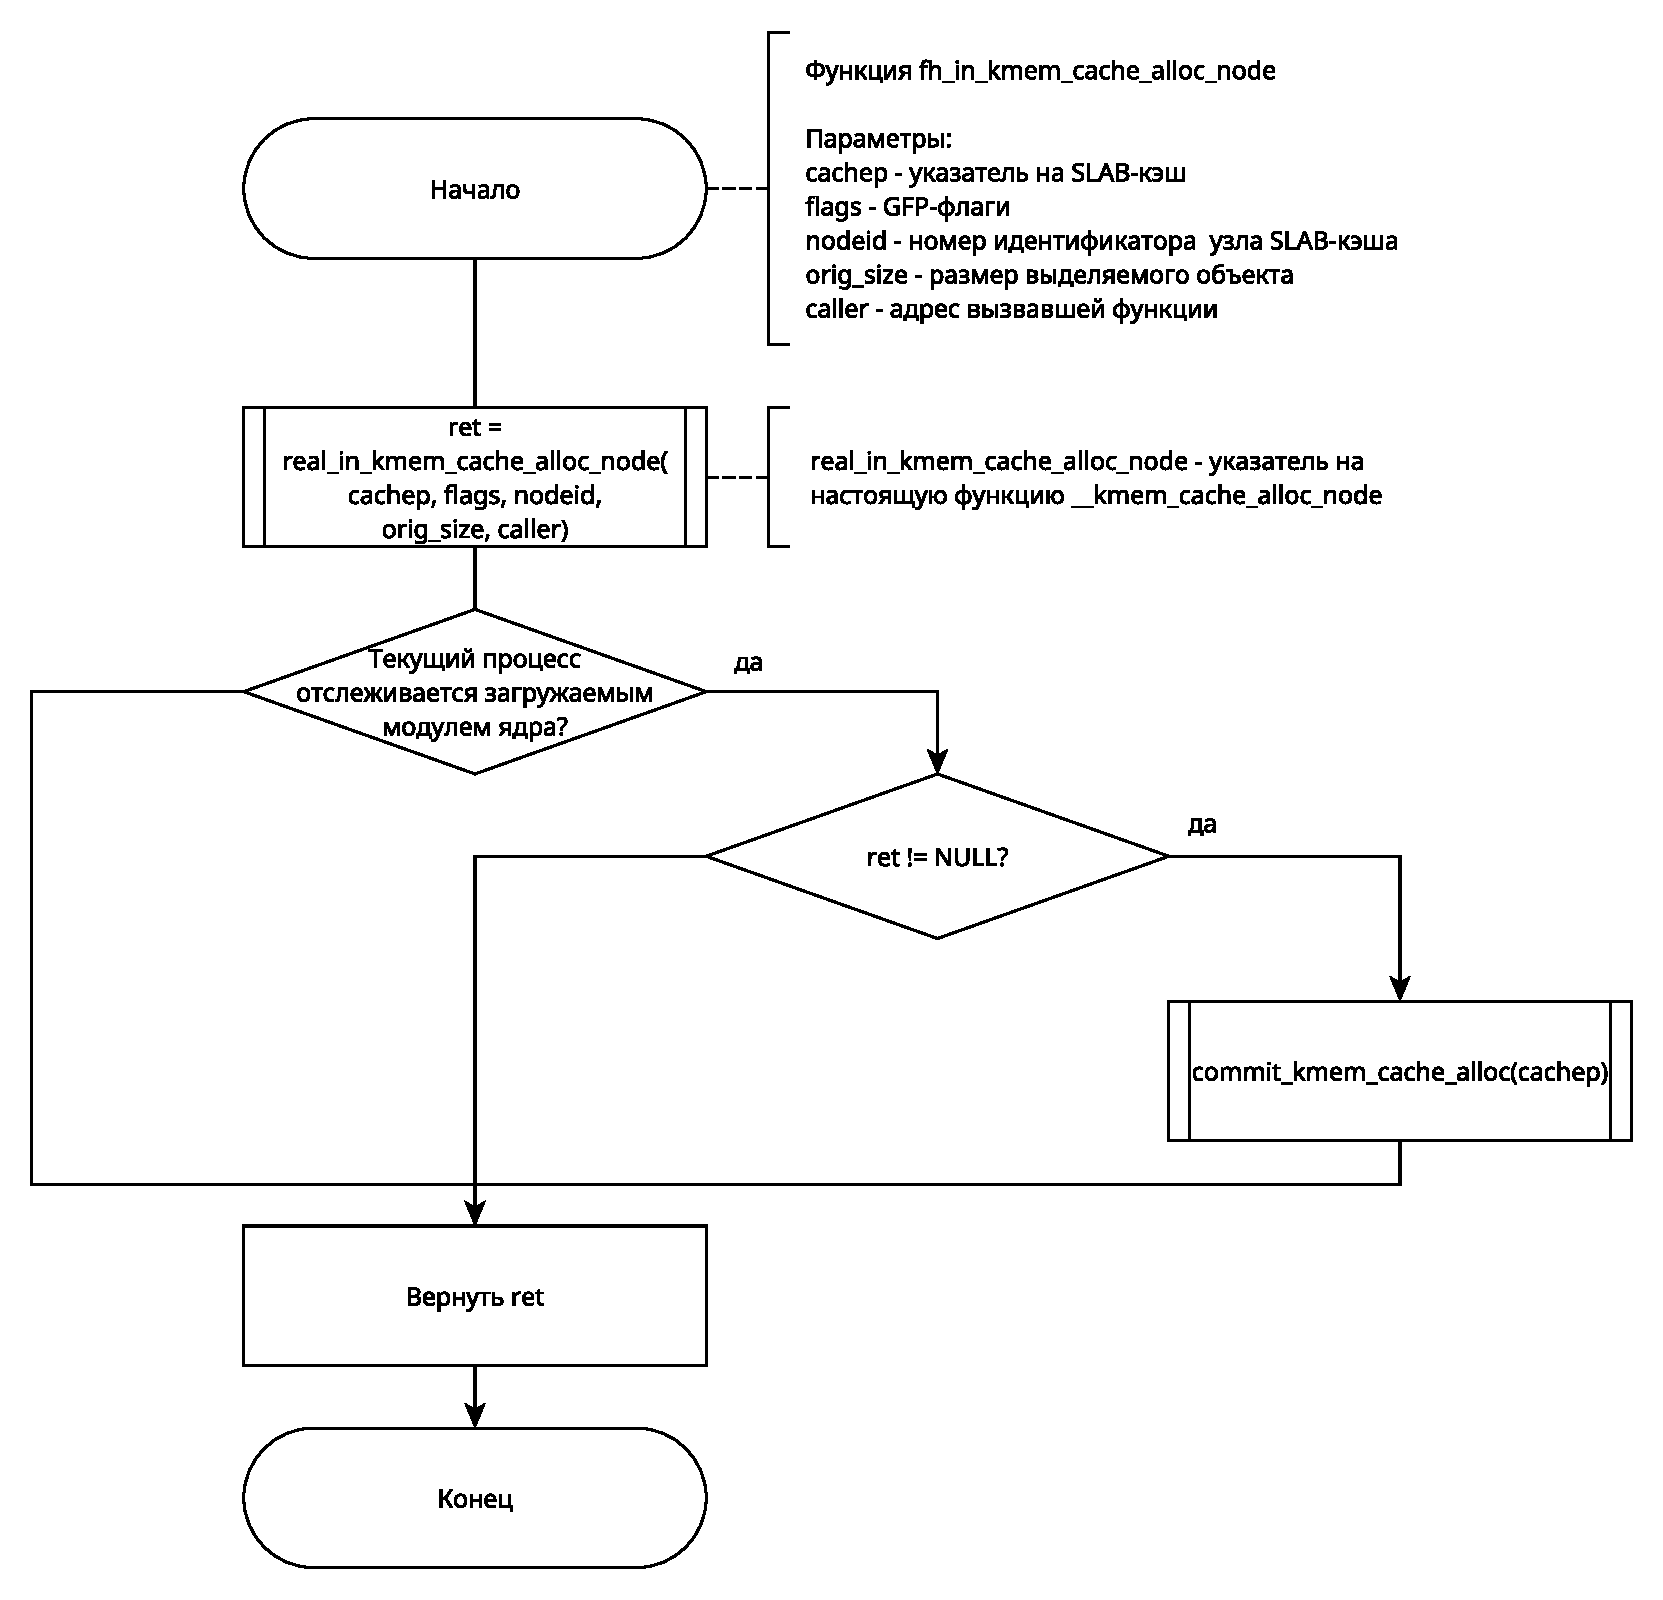
\includegraphics[width=0.6\linewidth]{fh_in_kmem_cache_alloc_node_alg}
	\caption{Схема алгоритма подменяемой функции для вызова \_\_kmem\_cache\_alloc\_node}
	\label{fh_in_kmem_cache_alloc_node_alg}
\end{figure}
\begin{figure}[H]
	\centering
	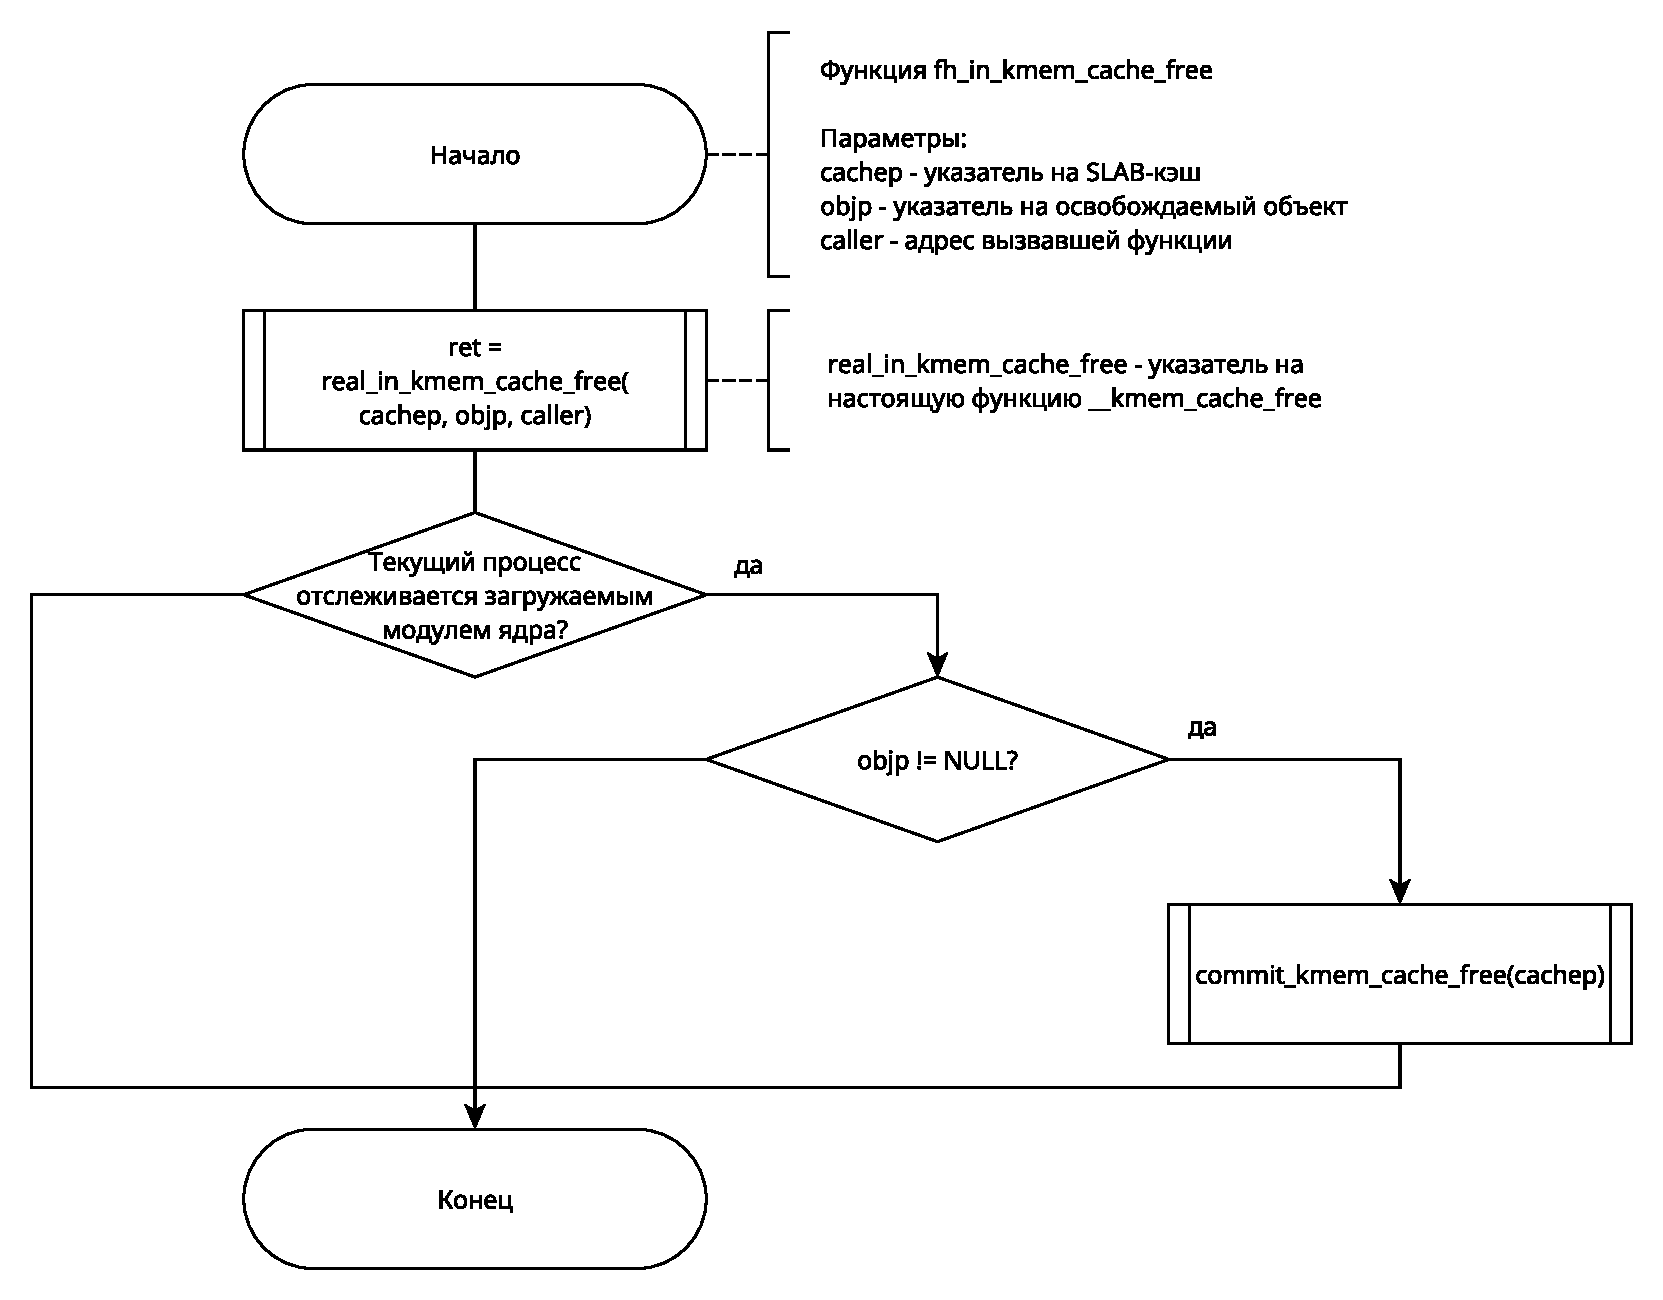
\includegraphics[width=0.6\linewidth]{fh_in_kmem_cache_free_alg}
	\caption{Схема алгоритма подменяемой функции для вызова \_\_kmem\_cache\_free}
	\label{fh_in_kmem_cache_free_alg}
\end{figure}
\begin{figure}[H]
	\centering
	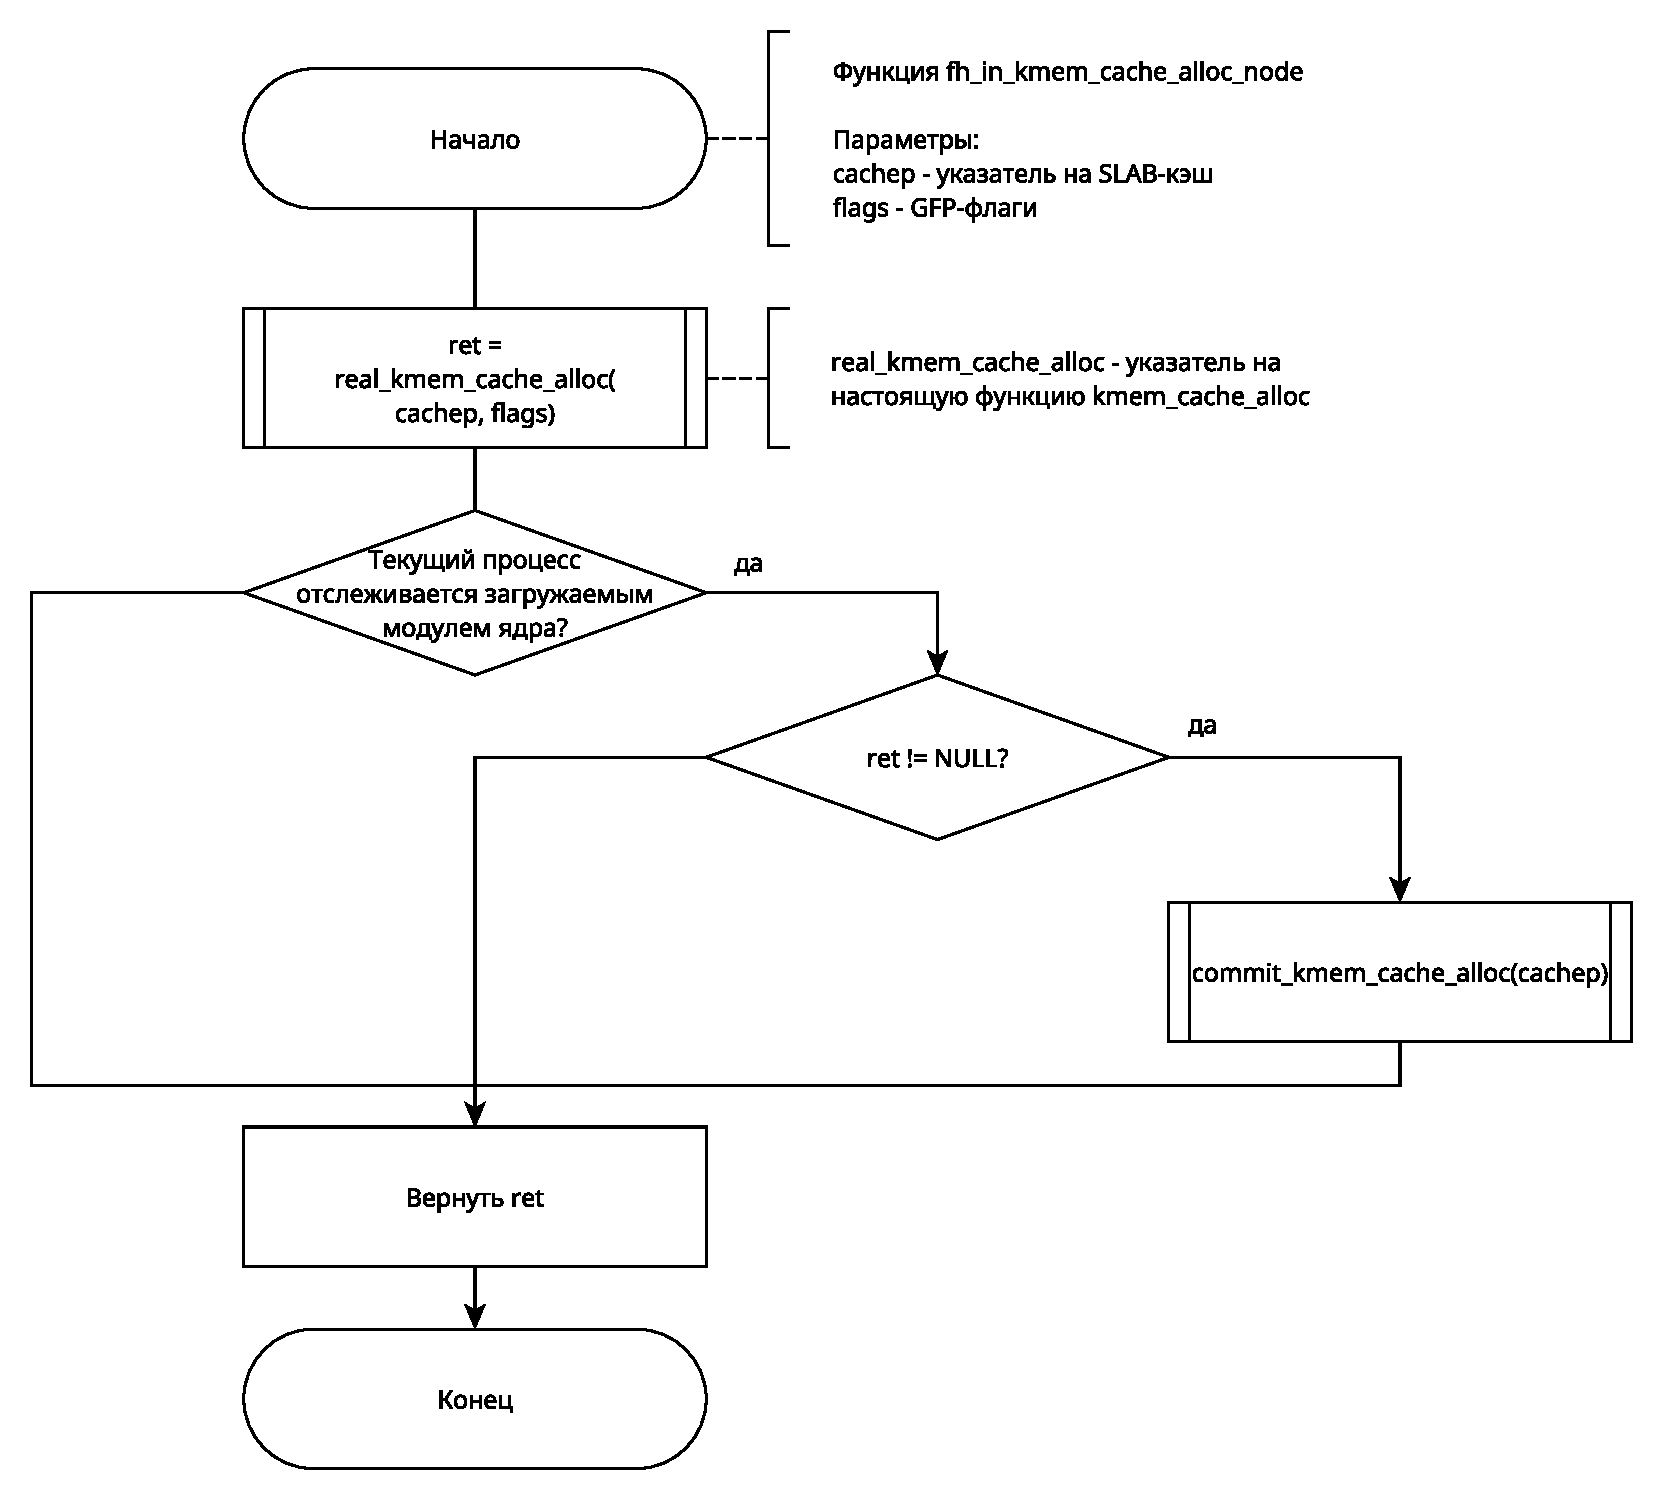
\includegraphics[width=0.6\linewidth]{fh_kmem_cache_alloc_alg}
	\caption{Схема алгоритма подменяемой функции для вызова kmem\_cache\_alloc}
	\label{fh_kmem_cache_alloc_alg}
\end{figure}
\begin{figure}[H]
	\centering
	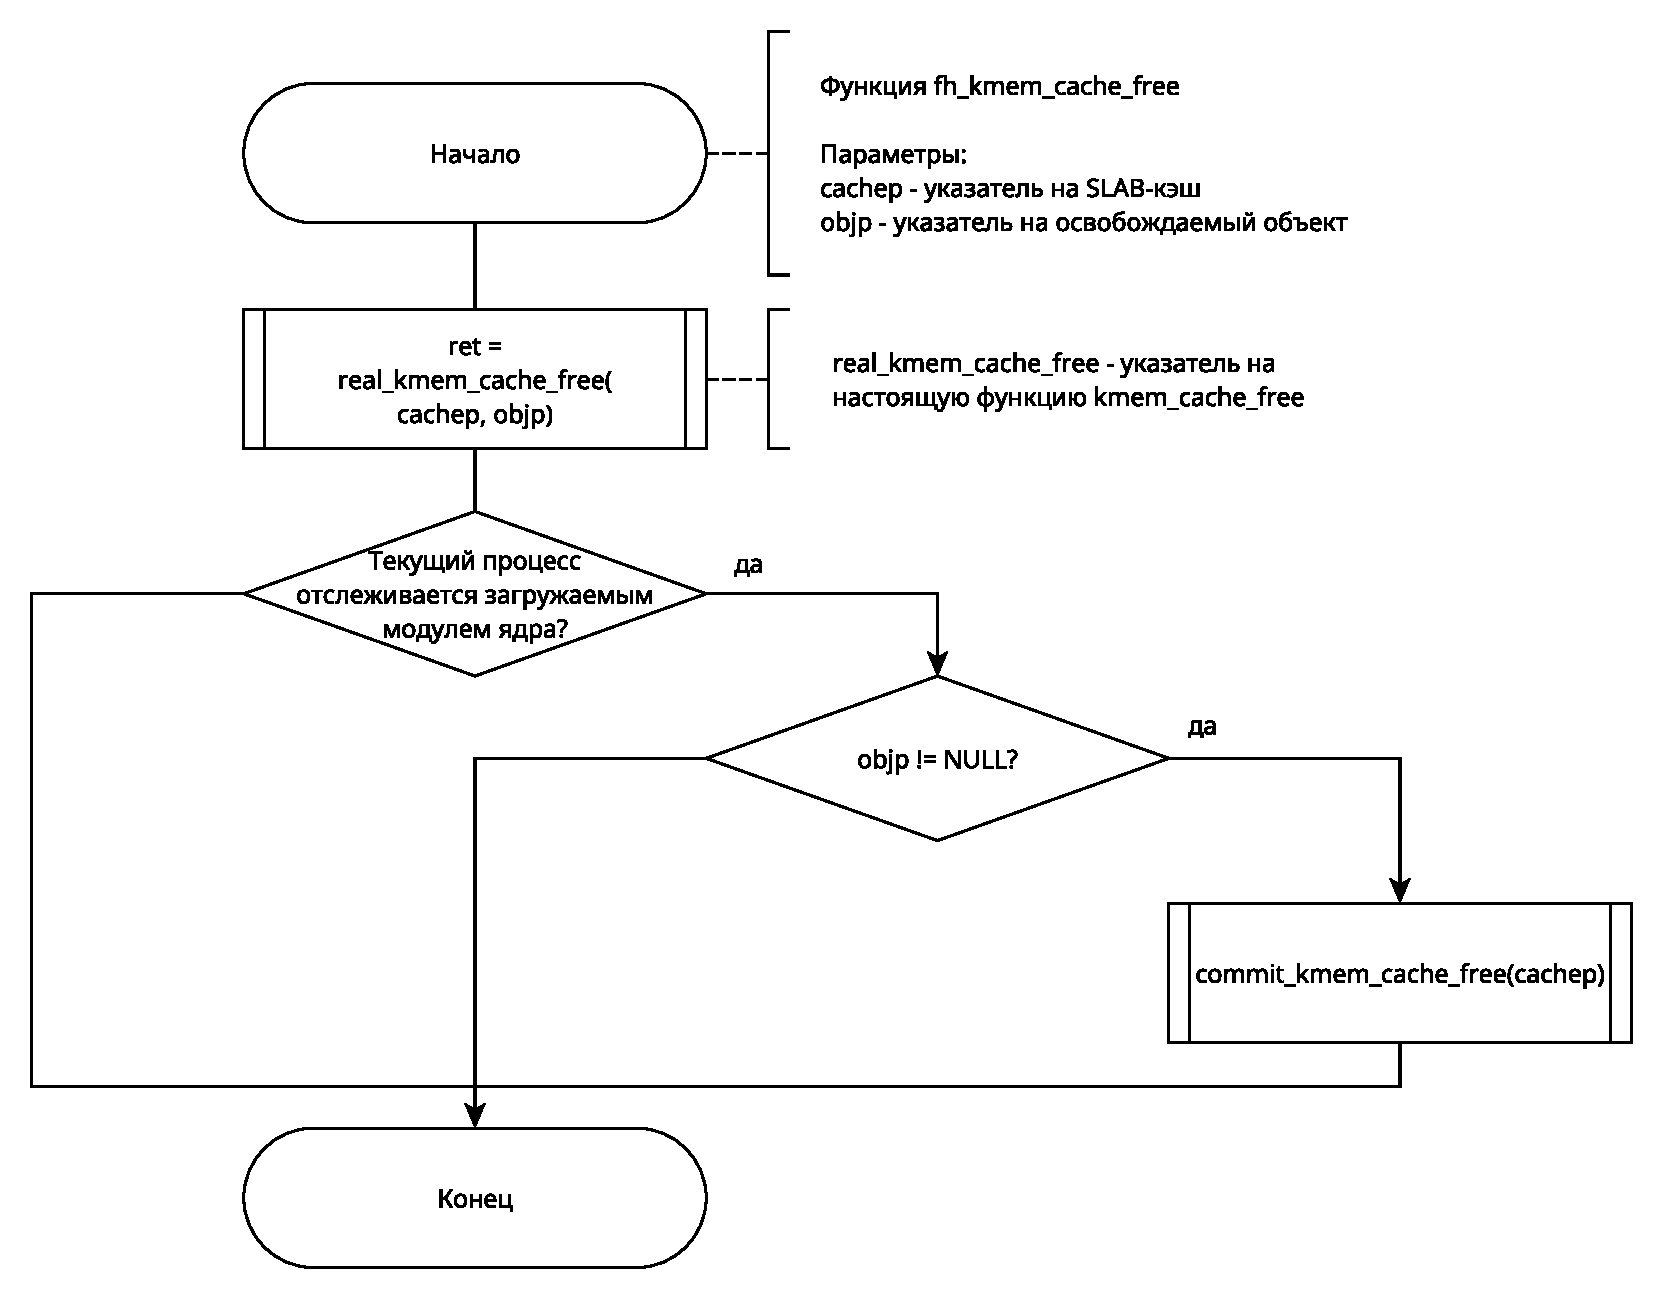
\includegraphics[width=0.6\linewidth]{fh_kmem_cache_free_alg}
	\caption{Схема алгоритма подменяемой функции для вызова kmem\_cache\_free}
	\label{fh_kmem_cache_free_alg}
\end{figure}
\begin{figure}[H]
	\centering
	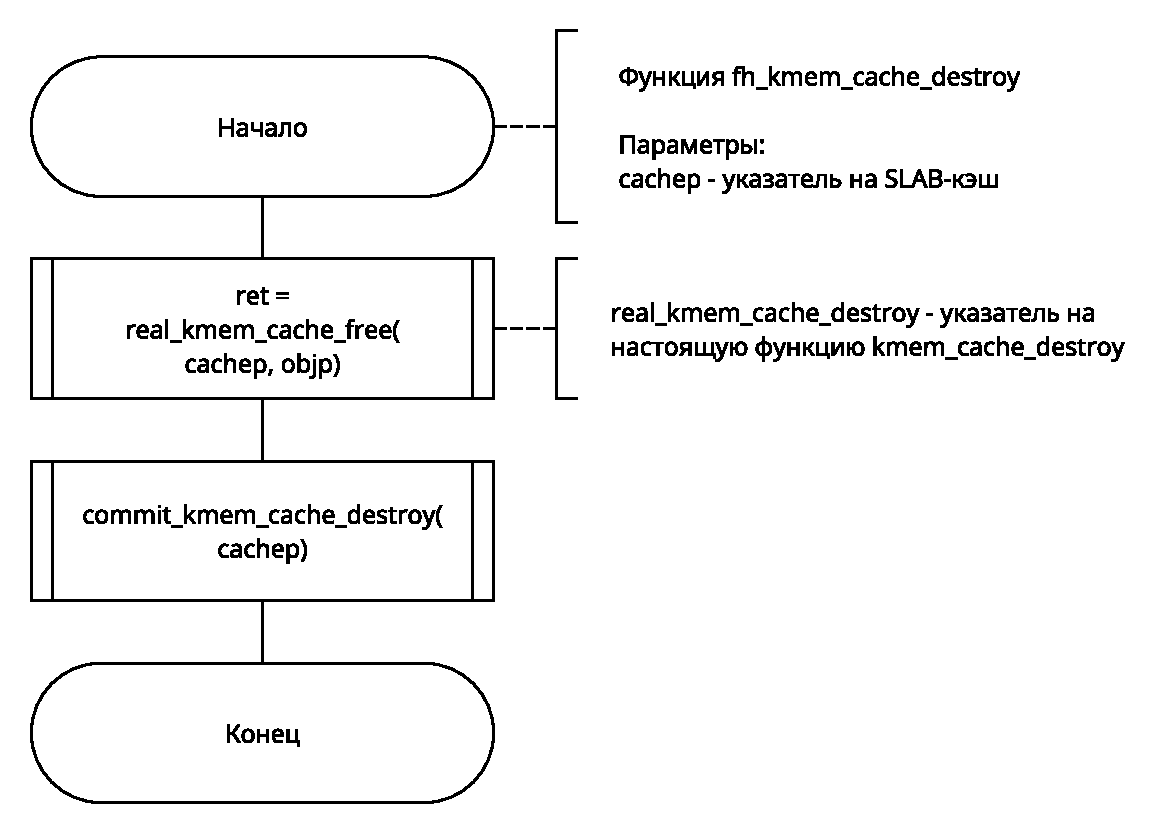
\includegraphics[width=0.6\linewidth]{fh_kmem_cache_destroy_alg}
	\caption{Схема алгоритма подменяемой функции для вызова kmem\_cache\_destroy}
	\label{fh_kmem_cache_destroy_alg}
\end{figure}
\begin{figure}[H]
	\centering
	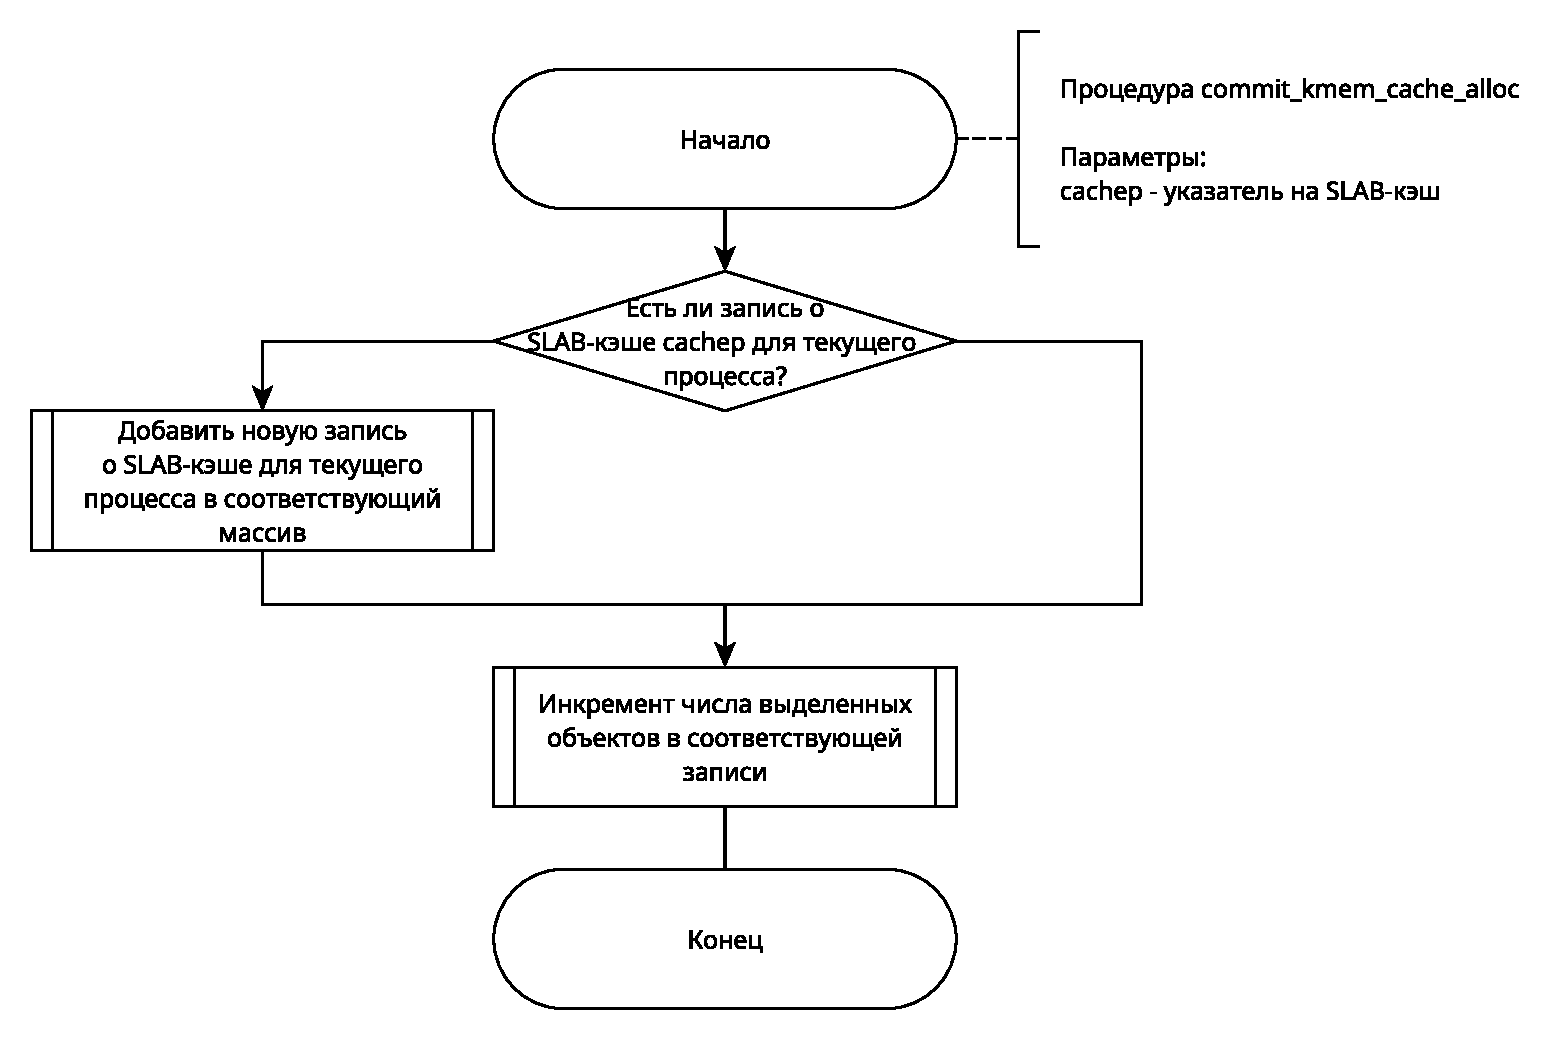
\includegraphics[width=0.6\linewidth]{commit_kmem_cache_alloc_alg}
	\caption{Схема алгоритма процедуры commit\_kmem\_cache\_alloc}
	\label{commit_kmem_cache_alloc_alg}
\end{figure}
\begin{figure}[H]
	\centering
	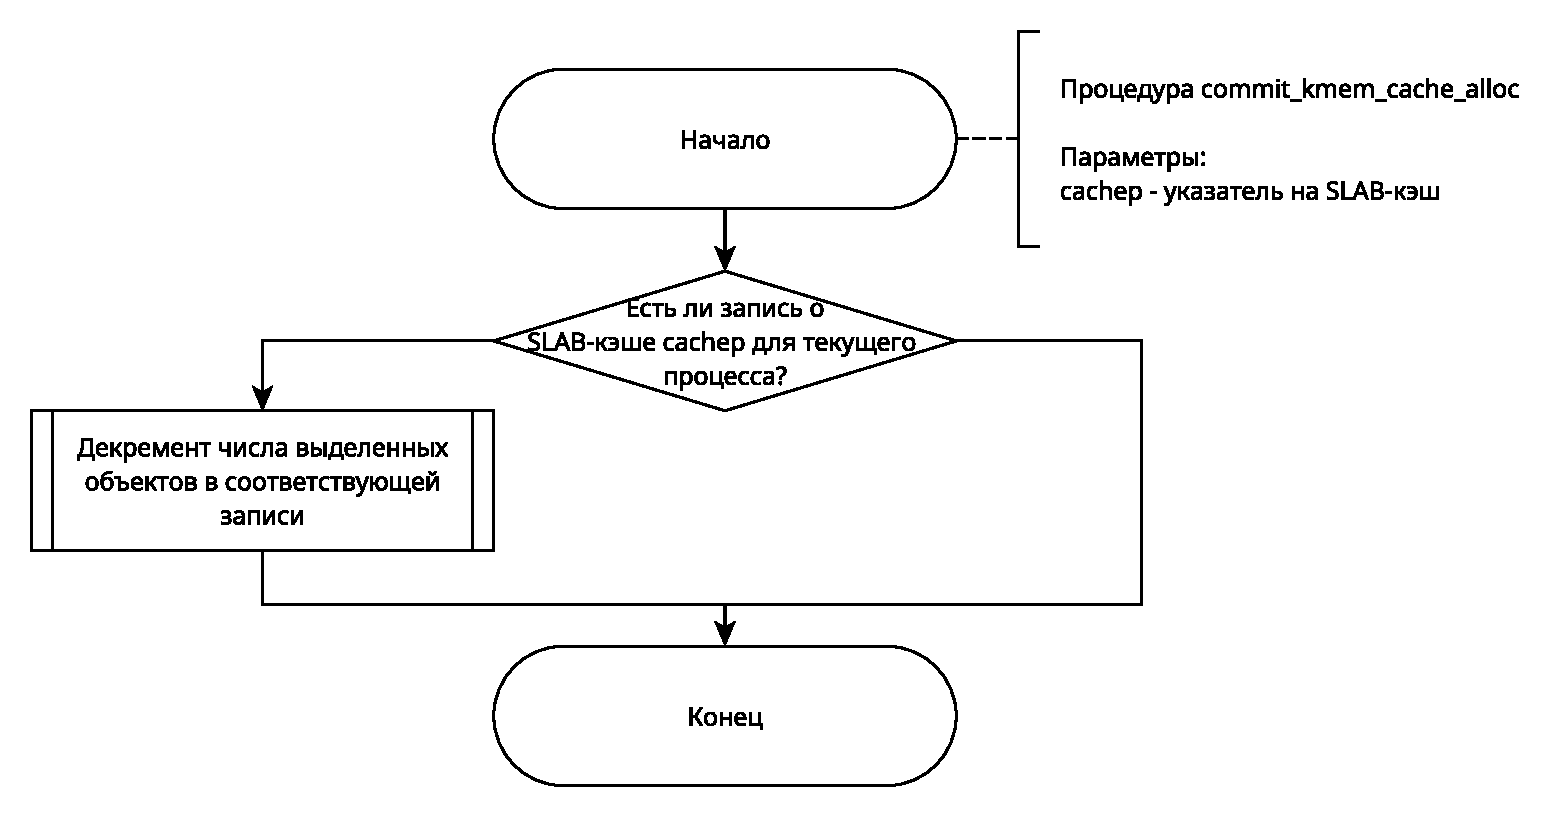
\includegraphics[width=0.6\linewidth]{commit_kmem_cache_free_alg}
	\caption{Схема алгоритма процедуры commit\_kmem\_cache\_free}
	\label{commit_kmem_cache_free_alg}
\end{figure}
\begin{figure}[H]
	\centering
	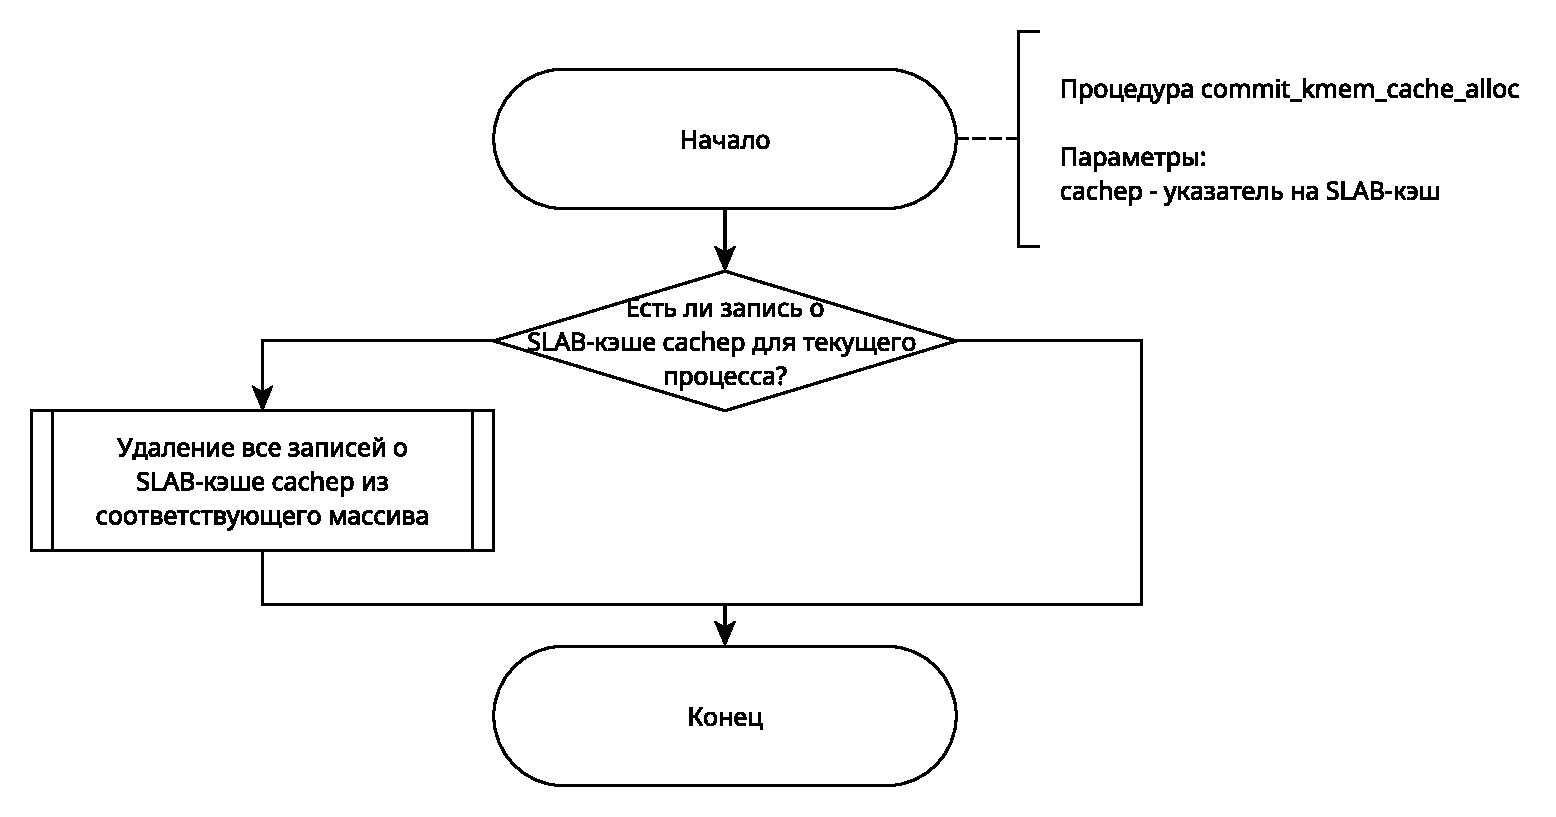
\includegraphics[width=0.6\linewidth]{commit_kmem_cache_destroy_alg}
	\caption{Схема алгоритма процедуры commit\_kmem\_cache\_destroy}
	\label{commit_kmem_cache_destroy_alg}
\end{figure}

\section*{Вывод}

Были разработаны последовательности преобразований в загружаемом модуле ядре для мониторинга использования SLAB-кэша процессами, алгоритмы загрузки и выгрузки разрабатываемого загружаемого модуля ядра, алгоритмы перехвата функции, чтения и записи для файла в виртуальной файловой системе proc и алгоритмы необходимых подменяемых функций.
